\documentclass[t, screen, aspectratio=43]{beamer}
\usepackage[T1]{fontenc}
\usepackage[utf8]{inputenc}
\usepackage{epsf}
\usepackage{graphicx}
\usepackage{geometry}
\usepackage{tabularx}
\usepackage[table]{colortbl}
\usepackage{xcolor}
\usepackage{soul}
\usepackage[normalem]{ulem}
\usepackage{tikz}
\usepackage{subcaption}
% Use the NTNU-temaet for beamer 
% \usetheme[style=ntnu|simple|vertical|horizontal, 
%     language=bm|nn|en, 
%     smalltitle, 
%     city=all|trondheim|alesund|gjovik]{ntnu2017}
\usetheme[style=helvet,language=en]{ntnu2017}

\usepackage[english]{babel}
\usepackage[style=numeric,backend=biber,natbib=false,sorting=none]{biblatex}

\title[Short title]{Ultra-Low Power PLL for Wake-up Receiver Applications}
\subtitle{Specialization Project Progress - 8th Week}
\author[C Nielsen]{Cole Nielsen}
\institute[NTNU]{Department of Electronic Systems, NTNU}
\date{18 October 2019 (Calendar week 42)}
%\date{} % To have an empty date

\addbibresource{example.bib} % Add bibliography database

% Set the reference style to numeric.
% See here: http://tex.stackexchange.com/questions/68080/beamer-bibliography-icon
\setbeamertemplate{bibliography item}[text] 

% Set bibliography fonts to a small size.
\renewcommand*{\bibfont}{\footnotesize}




\begin{document}

\begin{frame}
	\titlepage%
\end{frame}

% Alternatively, special title page command to get a different background
% \ntnutitlepage

% #############################################################################
% Timeline
% #############################################################################
\begin{frame}
	\frametitle{Autumn Timeline}
	\begin{table}[htb!]
		\tiny
		\centering
		\vspace{-1em}
		\def\arraystretch{1.5}		
		\setlength\arrayrulewidth{0.75pt}
		\setlength{\tabcolsep}{1em} % for the horizontal padding
		\begin{tabular}{|l|l|l|l|}
			\hline 
			\rule[-1ex]{0pt}{2.5ex} \cellcolor{gray!40}\textbf{Week} & \cellcolor{gray!40}\textbf{Dates} &\cellcolor{gray!40}\textbf{Tasks} & \cellcolor{gray!40}\textbf{Outcomes}\\ 
			\hline 
			\rule[-1ex]{0pt}{2.5ex} \cellcolor{red!20}\textbf{36}& \cellcolor{red!20}2.9 - 8.9 & \cellcolor{red!20}Review PLL Design & \cellcolor{red!20}Refreshed Knowledge\\ 
			\hline 
			\rule[-1ex]{0pt}{2.5ex} \cellcolor{red!20}\textbf{37}& \cellcolor{red!20}9.9 - 15.9 & \cellcolor{red!20}Modeling/simulation (set up) & \cellcolor{red!20}--\\ 
			\hline 
			\rule[-1ex]{0pt}{2.5ex} \cellcolor{red!20}\textbf{38}& \cellcolor{red!20}16.9 - 22.9 & \cellcolor{red!20}Modeling/simulation &\cellcolor{red!20}TDC/DCO Requirements\\ 
			\hline 
			\rule[-1ex]{0pt}{2.5ex} \cellcolor{red!20}\textbf{39}& \cellcolor{red!20}23.9 - 29.9& \cellcolor{red!20}Modeling/simulation& \cellcolor{red!20}Loop Filter/Digital Algorithms\\ 
			\hline 
			\rule[-1ex]{0pt}{2.5ex} \cellcolor{red!20}\textbf{40}& \cellcolor{red!20}30.9 - 6.10& \cellcolor{red!20}Modeling/simulation& \cellcolor{red!20}{Loop filter, DCO, TDC, calibration}\color{black}\\ 
			\hline 
			\rule[-1ex]{0pt}{2.5ex} \cellcolor{red!20}\textbf{41}&\cellcolor{red!20}7.10 - 13.10&\cellcolor{red!20}Circuit Research &\cellcolor{red!20}DCO/Divider topologies, Ideal Virtuoso implementation\\ 
			\hline 
			\rule[-1ex]{0pt}{2.5ex} \cellcolor{green!20}\textbf{42}&\cellcolor{green!20}14.10 - 20.10&\cellcolor{green!20}Circuit Research &\cellcolor{green!20}TDC/other topologies\\ 
			\hline 
			\rule[-1ex]{0pt}{2.5ex} \textbf{43}& 21.10 - 27.10& Circuit Implementation& Digital logic (schematic)\\ 
			\hline 
			\rule[-1ex]{0pt}{2.5ex} \textbf{44}& 28.10 - 3.11& Circuit Implementation& DCO (schematic)\\ 
			\hline 
			\rule[-1ex]{0pt}{2.5ex} \textbf{45}& 4.11 - 10.11& Circuit Implementation& Divider/other (schematic)\\ 
			\hline 
			\rule[-1ex]{0pt}{2.5ex} \textbf{46}& 11.11 - 17.11& Circuit Implementation (TDC)& \\ 
			\hline 
			\rule[-1ex]{0pt}{2.5ex} \textbf{47}& 18.11 - 24.11& Circuit Implementation (TDC)& TDC (schematic)\\ 
			\hline 
			\rule[-1ex]{0pt}{2.5ex} \textbf{48}& 25.11 - 1.12& Full Circuit testing & Testbenches, find bugs, design fixes\\ 
			\hline 
			\rule[-1ex]{0pt}{2.5ex} \textbf{49}& 2.12 - 8.12& Full Circuit testing& Design Fixes/iteration\\ 
			\hline 
			\rule[-1ex]{0pt}{2.5ex} \textbf{50}& 9.12 - 15.12& --& --\\ 
			\hline 
		\end{tabular}
		\begin{flushleft}\textbf{Legend:} \colorbox{red!20}{\textbf{Done}} \colorbox{green!20}{\textbf{Current}}  \colorbox{blue!20}{\textbf{Revised}}
		% *I will write the report simultaneously with the work.
		\end{flushleft}
		% \caption{Assigned specifications for branch line hybrid design.}
		% \label{asgn_specs}
	\end{table}   
\end{frame}


% #############################################################################
% This week
% #############################################################################

\begin{frame}
	\frametitle{Timeline Tasks}
	\begin{block}{This week}
		\begin{itemize}
			\footnotesize
			\item \textbf{TDC/Phase detector}
			\begin{itemize}
				\footnotesize
				\item New hybrid architecture using TDC and digital bang-bang phase detector to overcome resolution deficiencies.
				\item Already talked about topologies two weeks ago.
			\end{itemize} 
			\item \textbf{Python Simulation}:
			\begin{itemize}
				\footnotesize
				\item Variance of $K_{DCO}$ to analyze stability and effects on start-up.
				\item Added quantization to loop filter model.
				\item Added in hybrid TDC and digital bang-bang phase detector.
			\end{itemize} 
		\end{itemize}    
	\end{block}
\end{frame}

% #############################################################################
% sim/modeling approach
% #############################################################################

\begin{frame}
	\frametitle{TDC model limitations}
	\begin{block}{Continuous approximation model}
		\vspace{-0.5em}
		\center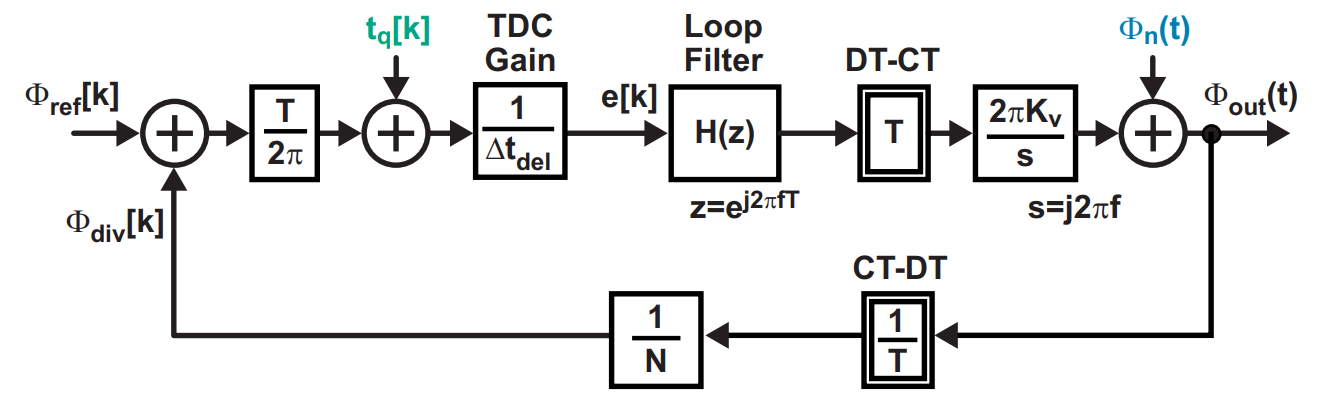
\includegraphics[width=0.6\textwidth, angle=0]{pll_loop.png}
		\begin{itemize}
			\scriptsize
			\item Have been using continuous approximation of PLL loop to model phase noise dynamics.
			\item Phase error here is \textit{instantly} available with added quantization noise.
			\item \textbf{Reality:} Low TDC resolution not manifested accurately.
			\begin{itemize}
				\scriptsize
				\item There is latency - Phase error must accumalate over many reference cycles until it is large enough to increment TDC by 1 LSB. 
			\end{itemize}		
			\item Time to increment 1 LSB for a frequency error $\Delta f$ is below. E.g. $\Delta f$ = 50 kHz, M=64, N=150 yields 47 $\mu s$ latency, or 750 reference cycles at 16 MHz. 
		\end{itemize} 
		\scriptsize	
		\begin{equation}
			t = \frac{N}{M\cdot\Delta f}
		\end{equation}
	\end{block}
\end{frame}

\begin{frame}
	\frametitle{Overcoming TDC limitations}
	\begin{block}{Issue of low TDC resolution}
		% \vspace{-0.5em}
		% \center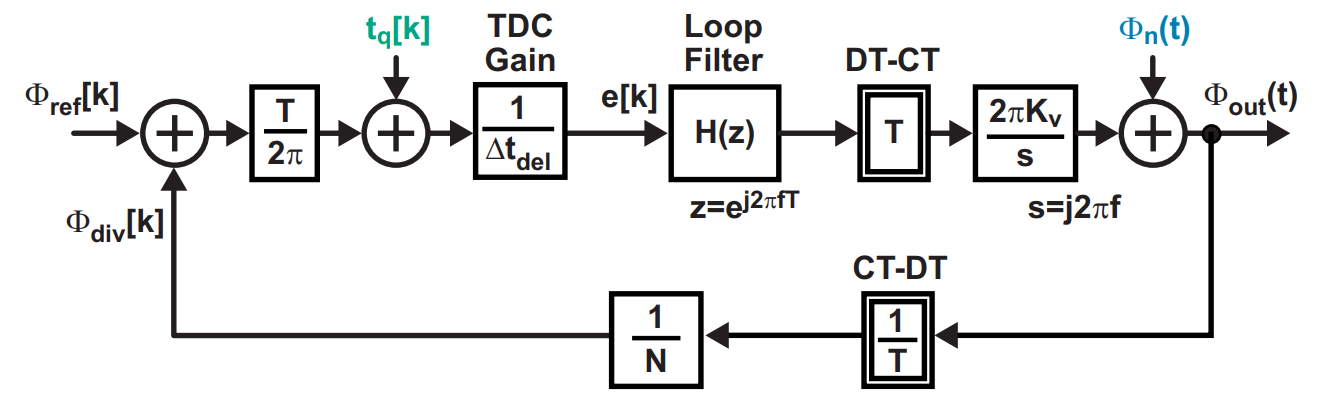
\includegraphics[width=0.6\textwidth, angle=0]{pll_loop.png}
		\begin{itemize}
			\scriptsize
			\item Low TDC resolution limits ability to track random phase walk (principal phase noise component).
			\item \textbf{TDC steps M} $>>$ \textbf{Divider N} for TDC response time to frequency error $\Delta f$ to be much less than period of $\Delta f$. This allows for the frequency error due to phase walk to be corrected before it contributes to the phase noise spectrum.
			\item If N=150, TDC bits $>>$ 7.2. 
			\begin{itemize}
				\scriptsize
				\item This is impractical. 
				\item Delay line TDC with ca. 150 stages would be problematic.
				\item Counter based TDC limited to exactly M=N.
			\end{itemize}		
		\end{itemize} 
	\end{block}
\end{frame}

\begin{frame}
	\frametitle{Overcoming TDC limitations}
	\begin{block}{Bang-bang phase detector}
		\vspace{-0.5em}
		\center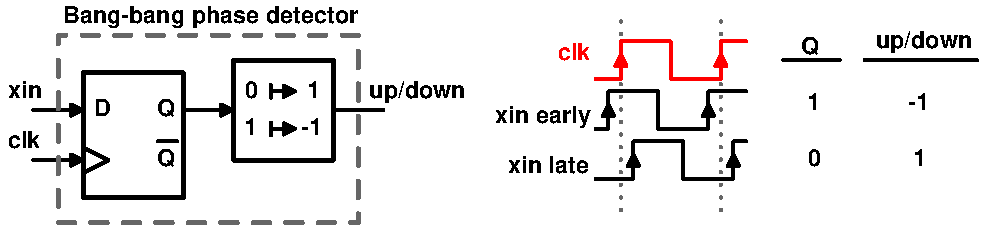
\includegraphics[width=0.7\textwidth, angle=0]{bang_bang3.pdf}
		\begin{itemize}
			\scriptsize
			\item Need a way to incorporate more instantaneous phase feedback, enter the \textbf{bang-bang phase detector} (BB-PD).
			\begin{itemize}
				\scriptsize
				\item Bang-bang detector samples every cycle, measuring if the input edge is late or early relative to the clock. 
			\end{itemize}	
			\item Basic implementation is a D flip-flop.
			\item To correct phase error (if small in magnitude):
			\begin{itemize}
				\scriptsize
				\item Early input $\rightarrow$ decrement oscillator frequency
				\item Late input $\rightarrow$ incremenent oscillator frequency
			\end{itemize}
		\end{itemize} 
	\end{block}
\end{frame}



\begin{frame}
	\frametitle{Overcoming TDC limitations}
	\begin{block}{Hybrid detector}
		\center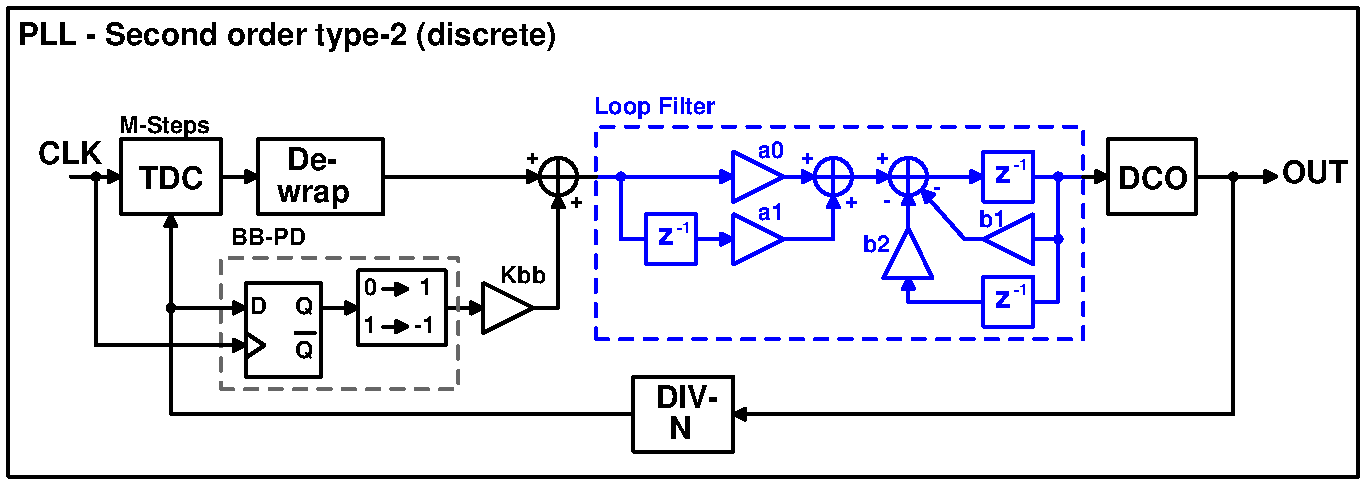
\includegraphics[width=0.7\textwidth, angle=0]{pll_sec_order_bb.pdf}
		\begin{itemize}
			\scriptsize
			\item Combine TDC and bang-bang phase detector to yield better overall phase detector.
			\begin{itemize}
				\scriptsize
				\item TDC good for achieving fast lock with large frequency offset.
				\item Bang-bang good for steady-state tracking. 
			\end{itemize}	
			\item In phase error signal, TDC sets integer part of signal, BB-PD is fractional.
			\begin{itemize}
				\scriptsize
				\item Near steady state, TDC signal is 0, so BB-PD dominates.
			\end{itemize}	
			\item Remainder of PLL is same as before.
		\end{itemize}	
	\end{block}
\end{frame}

\begin{frame}
	\frametitle{Overcoming TDC limitations}
	\begin{block}{Example TDC out with low resolution.}
		\begin{itemize}
			\scriptsize
			\item Simulated 2.4 GHz PLL, with 16 MHz reference, 50 kHz bandwidth, 64 TDC steps.
			\item Does a good job locking from large offset, bad phase error in steady state.
			\item Noticably no tracking of small phase variations (phase noise) in steady state.
		\end{itemize} 	

		\center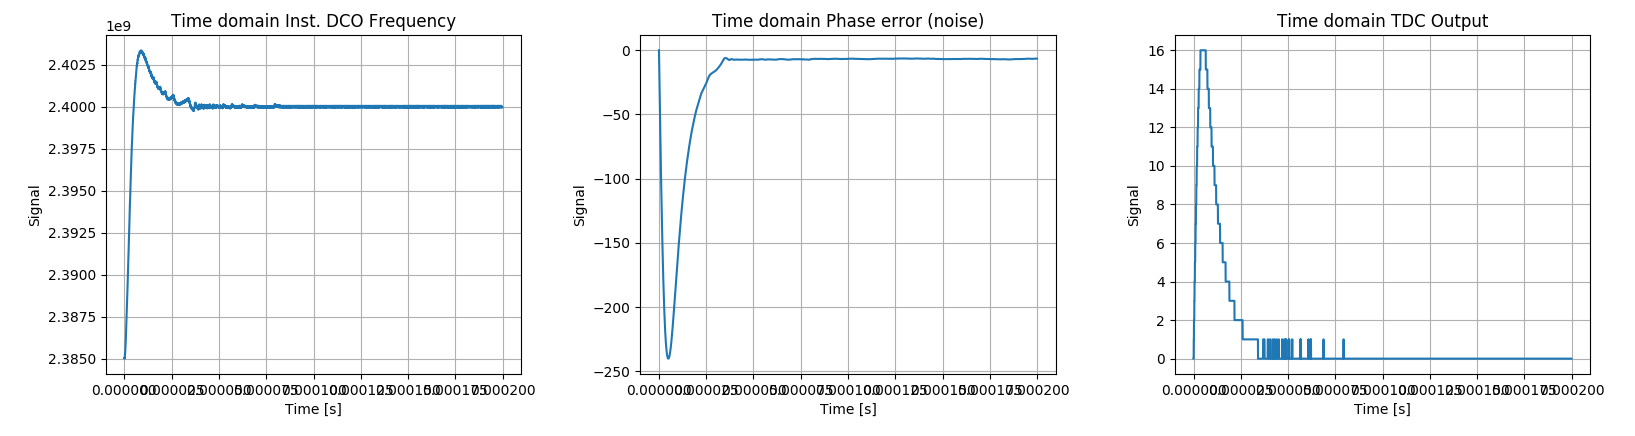
\includegraphics[width=1.0\textwidth, angle=0]{pllsim.png}
	\end{block}
\end{frame}

\begin{frame}
	\frametitle{Overcoming TDC limitations}
	\begin{block}{BB-PD with counter-based TDC}
		\center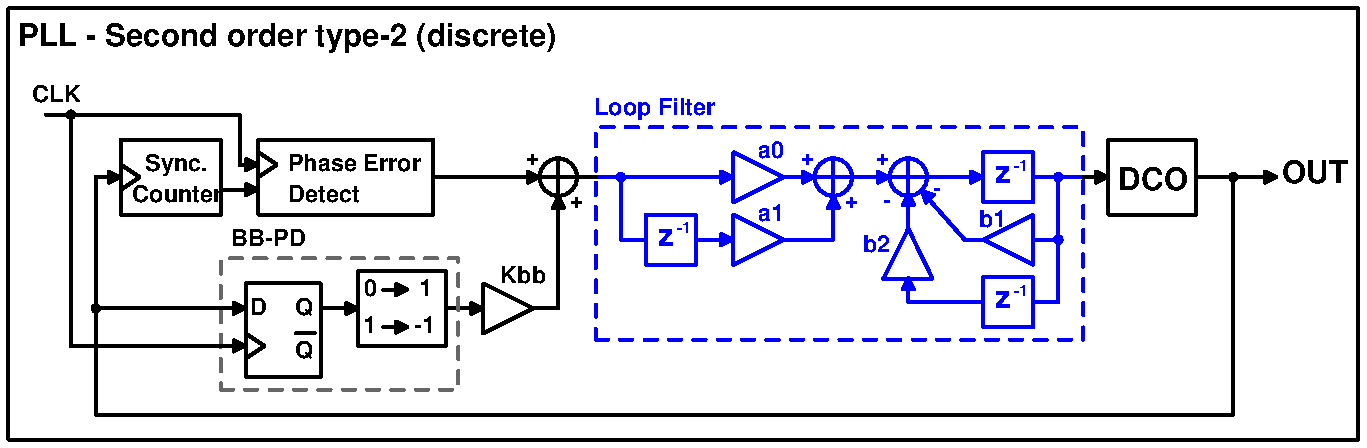
\includegraphics[width=0.7\textwidth, angle=0]{pll_sec_order_bb_counter.pdf}
		\begin{itemize}
			\scriptsize
			\item Counter-based TDC has no divider, connect BB-PD direct to DCO output.
			\item Disable synchronous counter and only use BB-PD near lock to save power?
		\end{itemize}	
	\end{block}
\end{frame}

\begin{frame}
	\frametitle{Overcoming TDC limitations}
	\begin{block}{BB-PD gain selection}
	\vspace{-0.5em}
		\center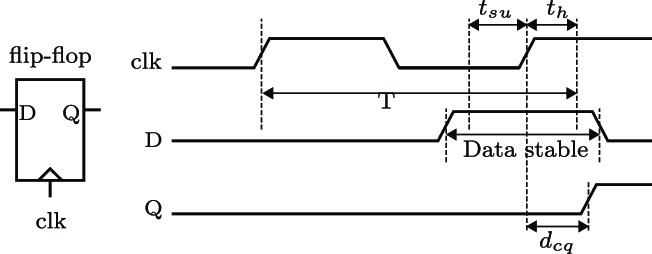
\includegraphics[width=0.5\textwidth, angle=0]{ff_setup_hold.png}
		\begin{itemize}
			\scriptsize
			\item Regardless of phase error magnitude, BB-PD output will be fixed magnitude. How do we set $K_{BB}$?
		\begin{itemize}
			\scriptsize
			\item To achieve maximum resolution (lowest phase noise), $K_{BB}$ should be defined by the minimum time difference resolvable by the BB-PD.
			\item If faster settling is need, increase $K_{BB}$
		\end{itemize}	
		\item Minimum effective temporal resolution of BB-PD is given by set-up and hold time requirements of flip-flop for deterministic output. So for use with a M-step TDC:
		\end{itemize}	
	\tiny
	\begin{equation}
		K_{BB} \geq M\cdot f_{clk}(t_{su}+t_{h})
	\end{equation}
	\end{block}
\end{frame}


\begin{frame}
	\frametitle{PLL Simulation with BB-PD}
	\begin{block}{Counter based TDC/divider.}
			\scriptsize
			- $f_{clk}$ = 16 MHz, N = 150 (2.4 GHz), 48 MHz initial offset, $t_{su} = t_h = 20 ps$.
	        \begin{tikzpicture}
	            \node[anchor=south west,inner sep=0] (image) at (0,0) {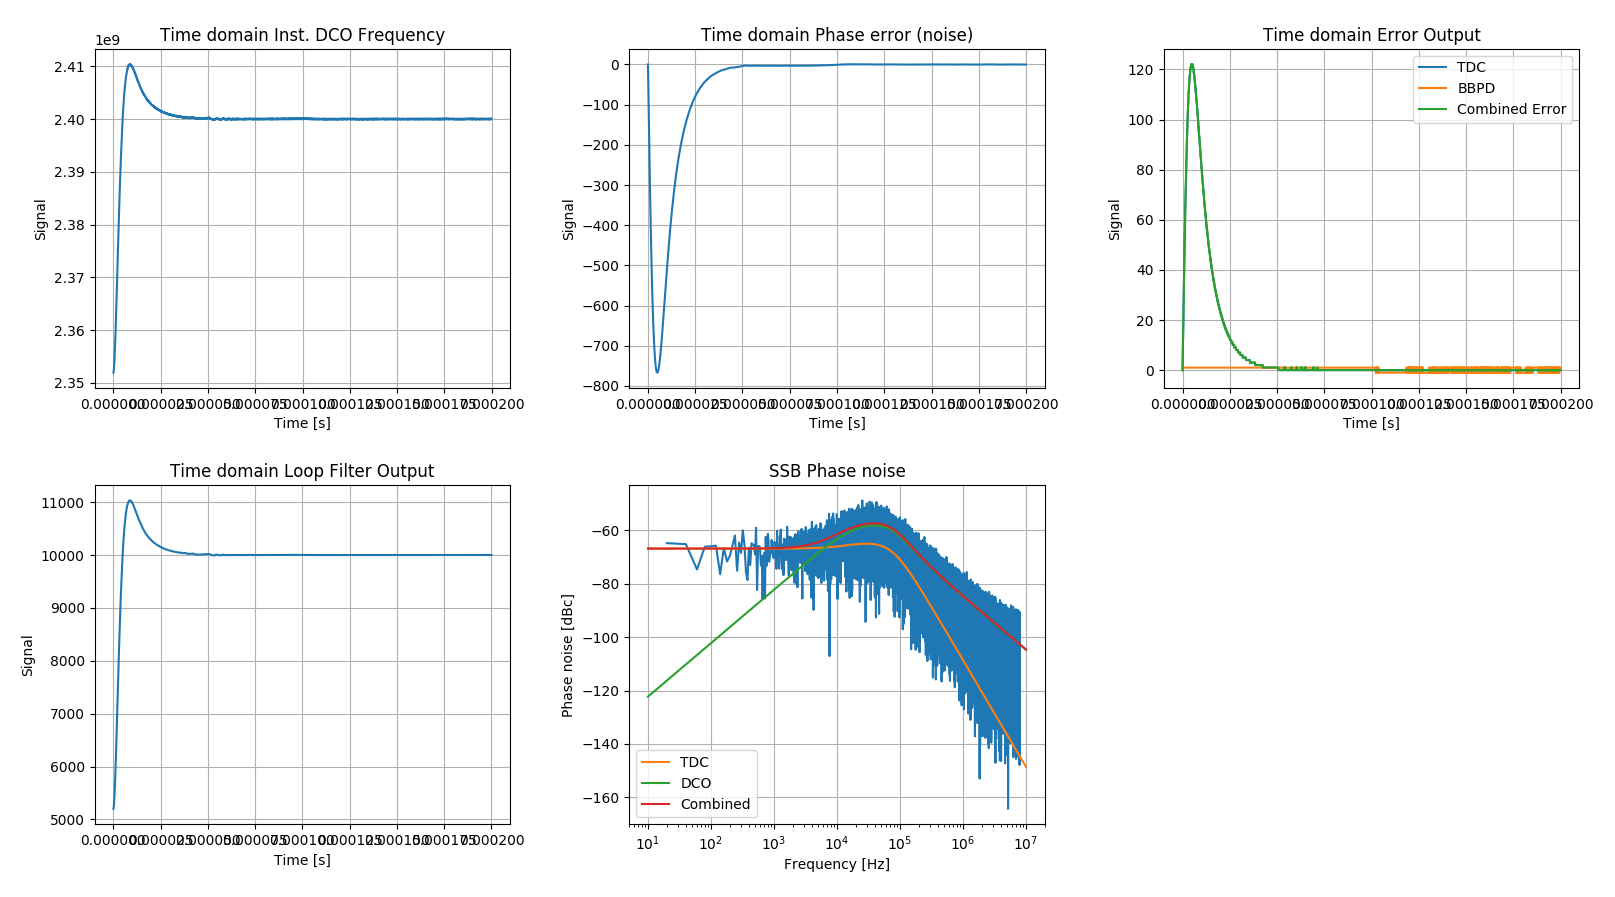
\includegraphics[width=0.95\textwidth]{pllsim_counter_bbpd.png}};
				\node[overlay, red,font={\bfseries\scriptsize}] at (9.5,1.5) {Phase noise matches model.};
	        \end{tikzpicture}
	\end{block}
\end{frame}


\begin{frame}
	\frametitle{PLL Simulation with BB-PD}
	\begin{block}{Delay line based TDC.}
			\scriptsize
			- TDC steps = 64, $f_{clk}$ = 16 MHz, N = 150 (2.4 GHz), 15 MHz initial offset, $t_{su} = t_h = 20 ps$.
			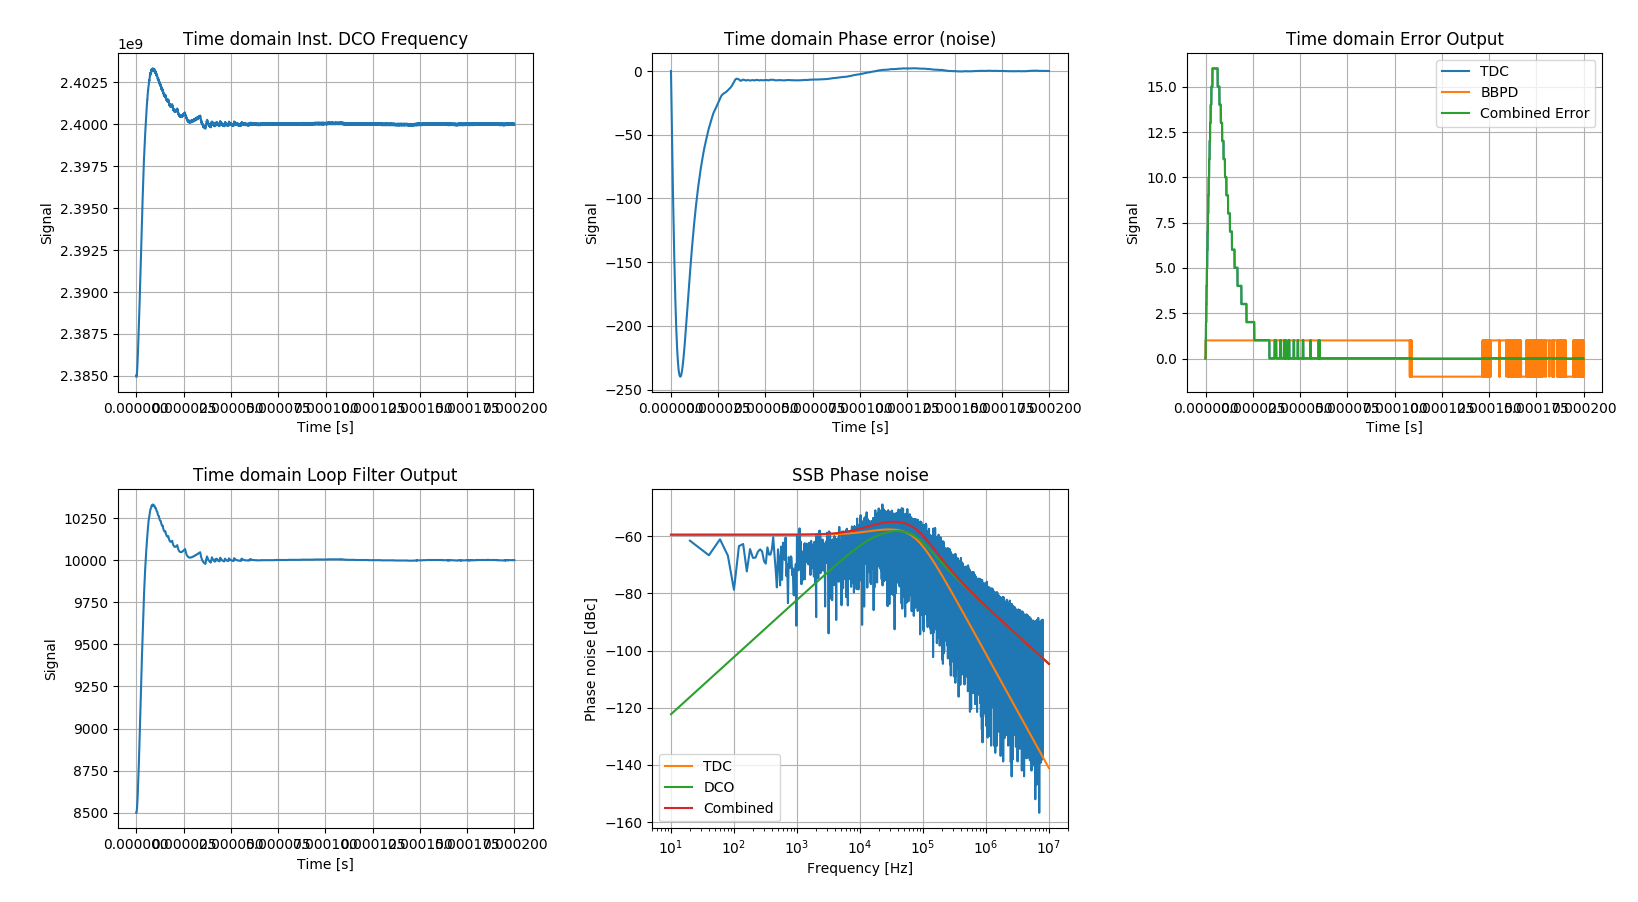
\includegraphics[width=0.95\textwidth, angle=0]{pllsim_fixed_bbpd.png}
	\end{block}
\end{frame}

\begin{frame}
	\frametitle{PLL Simulation with BB-PD}
	\begin{block}{Phase noise comparison with and without BB-PD.}
			\scriptsize
			- The discrepencies I saw last week between model and simulation were from the phase detector, not a math error.

		\begin{figure}[htb!]
	        \centering
	        \begin{subfigure}{.5\textwidth}
	            \centering
	            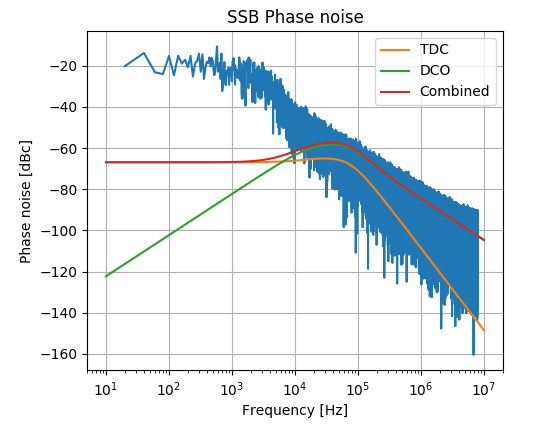
\includegraphics[width=0.9\linewidth]{old_pn.png}
	            \caption{\scriptsize Without BB-PD.}
	            \label{fig:rosc_3stg_cir}
	        \end{subfigure}%
	        \begin{subfigure}{.5\textwidth}
	            \centering
	            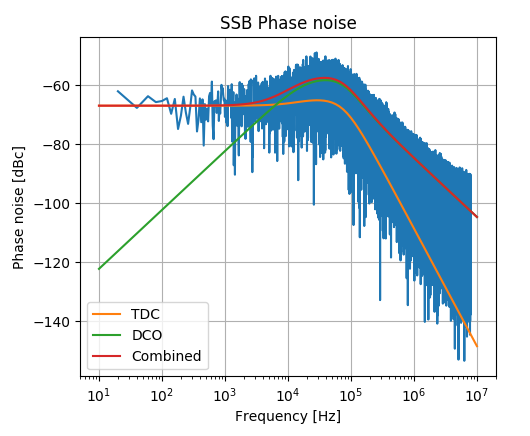
\includegraphics[width=0.9\linewidth]{new_pn_bbpd.png}
	            \caption{\scriptsize With BB-PD.}
	            \label{fig:rosc_3stg_wave}
	        \end{subfigure}
	        % \caption{Approximate model for ring oscillator inverter delay cell.}
	        \label{fig:rosc_3stg}
	    \end{figure}

	\end{block}
\end{frame}


\begin{frame}
	\frametitle{PLL Sim. - Datapath resolution}
	\begin{block}{Comparison of Counter PLL with 6-10 fractional bits.}
			\scriptsize
		\begin{itemize}
			\item Simulated PLL with various number of fractional bits in fixed point numeric representations. Number of integer bits varies.
		\end{itemize}

		\begin{figure}[htb!]
	        \centering
	        \begin{subfigure}{.33\textwidth}
	            \centering
	            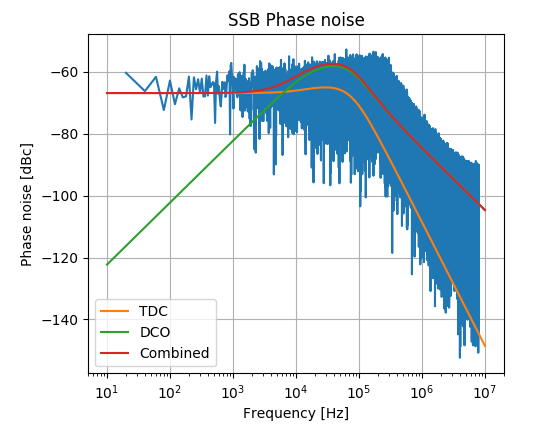
\includegraphics[width=1\linewidth]{6bit_frac_pn.png}
	            \caption{\scriptsize 6 Fractional bits.}
	            \label{fig:rosc_3stg_cir}
	        \end{subfigure}%
	        \begin{subfigure}{.33\textwidth}
	            \centering
	            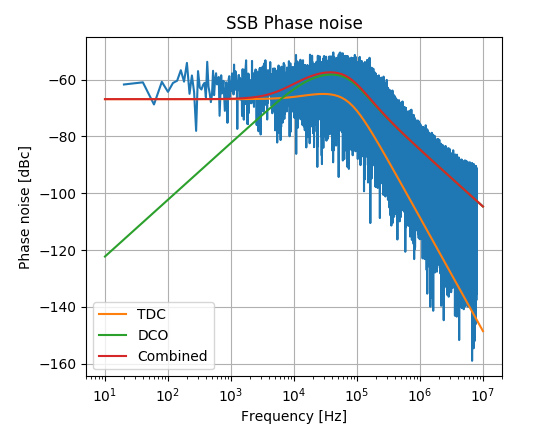
\includegraphics[width=1\linewidth]{8bit_frac_pn.png}
	            \caption{\scriptsize 8 Fractional bits.}
	            \label{fig:rosc_3stg_wave}
	        \end{subfigure}
	       	\begin{subfigure}{.33\textwidth}
	            \centering
	            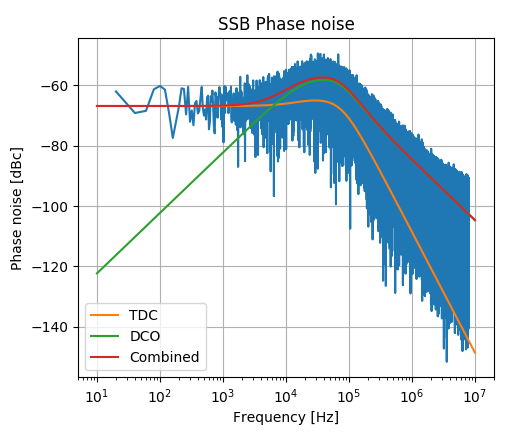
\includegraphics[width=1\linewidth]{10bit_frac_pn.png}
	            \caption{\scriptsize 10 Fractional bits.}
	            \label{fig:rosc_3stg_wave}
	        \end{subfigure}
	        % \caption{Approximate model for ring oscillator inverter delay cell.}
	        \label{fig:rosc_3stg}
	    \end{figure}
	\end{block}
\end{frame}


\begin{frame}
	\frametitle{PLL Sim. - Datapath resolution}
	\begin{block}{Resolution for fractional part from last week}
		\center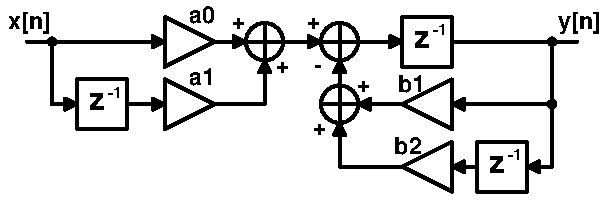
\includegraphics[width=0.4\textwidth, angle=0]{discrete_filter2.pdf}
		\begin{itemize}
			\scriptsize
			\item Last week came up with this expression based on the difference equation coefficients:
	    \begin{equation}
			\textnormal{\# Fractional bits} > \lceil -\log_2(a_0+a_1) \rceil
		\end{equation}
			\scriptsize
			\item For the configuration tested, 9 bits is the minimum based on the above equation. This seems to be in agreement with the simulation.
		\end{itemize} 	
	\end{block}
\end{frame}



\begin{frame}
	\frametitle{Simulation - Variation}
	\begin{block}{KDCO variation.}
			\scriptsize
		\begin{itemize}
			\item Simulated PLL with $K_{DCO}$ subject to variance, where $\sigma_{KDCO}$ is 20\% of nominal $K_{DCO}$.
			\item Stable with 50 runs.
		\end{itemize}
			\center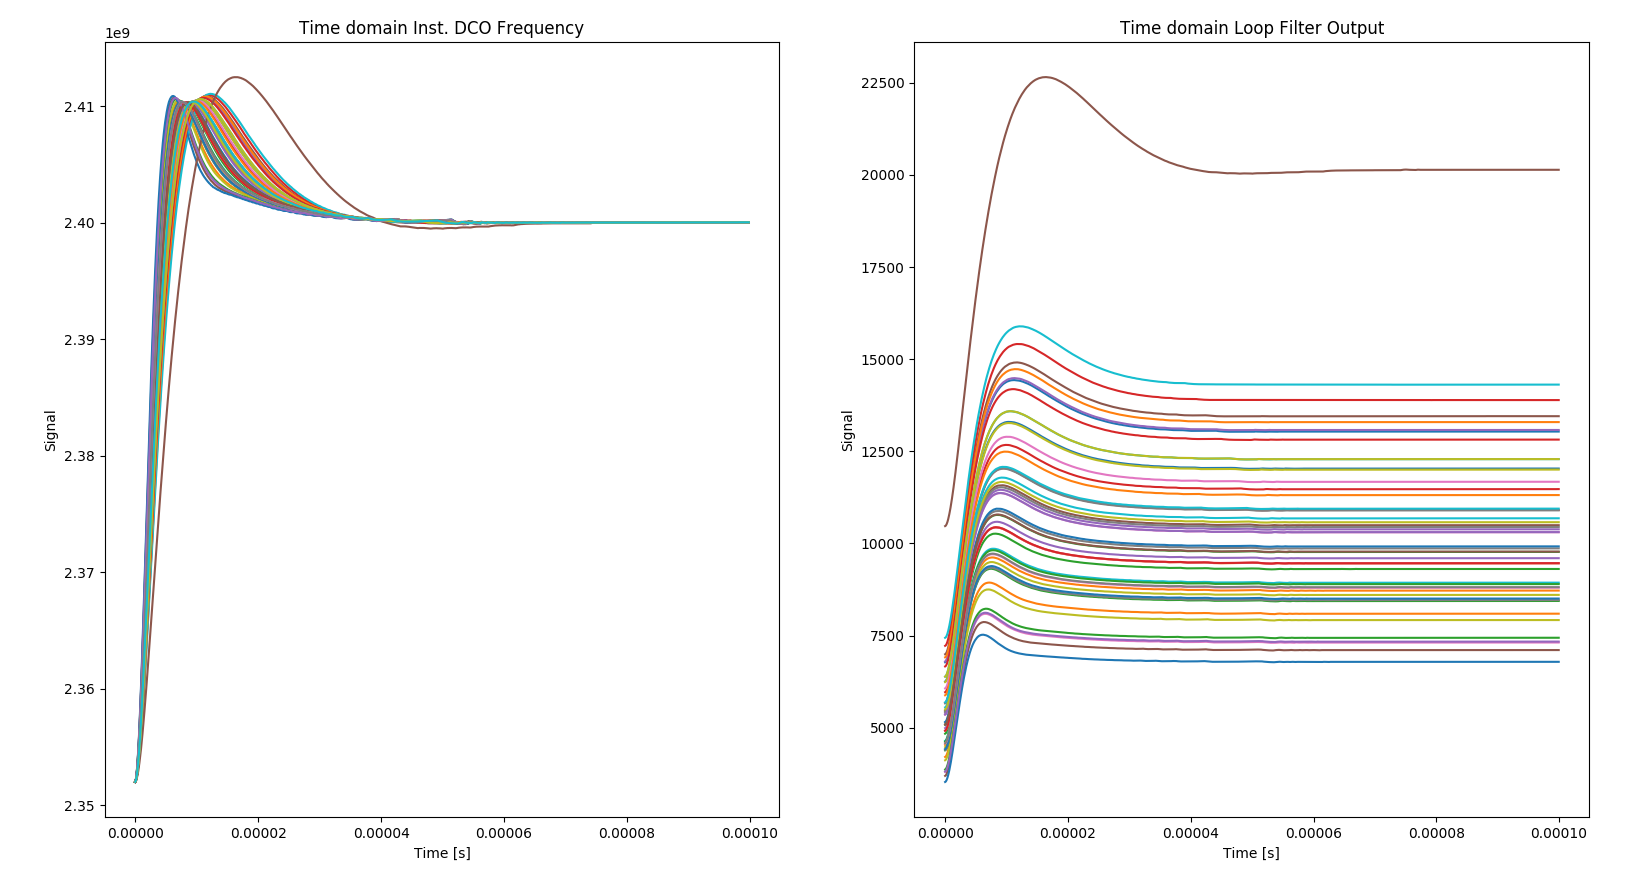
\includegraphics[width=0.8\textwidth, angle=0]{kdco_sweep.png}
	\end{block}
\end{frame}


\begin{frame}
	\frametitle{Simulation - Variation}
	\begin{block}{KDCO and initial frequency variation.}
			\scriptsize
		\begin{itemize}
			\item Simulated PLL with $K_{DCO}$ subject to variance, where $\sigma_{KDCO}$ is 20\% of nominal $K_{DCO}$.
			\item $f_{initial} = f_0 - \Delta f$ is subject to variance, where $\sigma_{\Delta f}$ is 1\% of nominal $f_0$.
			\item Stable with 50 runs.
		\end{itemize}
			\center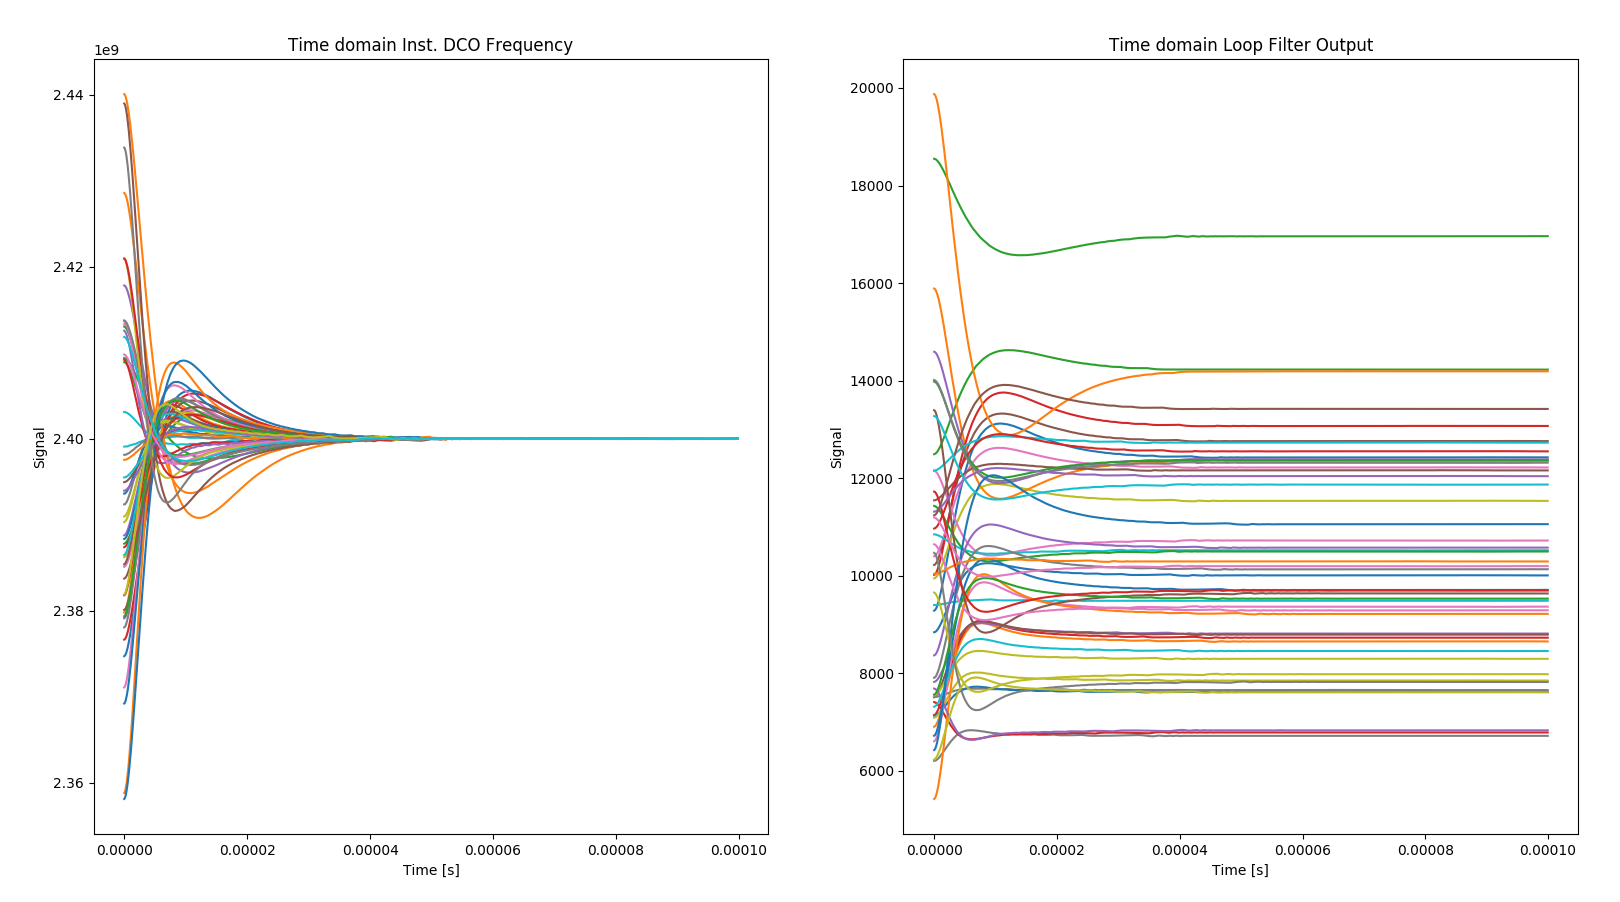
\includegraphics[width=0.7\textwidth, angle=0]{kdco_var_fstart_var.png}
	\end{block}
\end{frame}


% #############################################################################
% Loop Dynamics (continuous)
% #############################################################################

% \begin{frame}
% 	\frametitle{Loop Dynamics}
% 	\begin{block}{Still To Do}
% 		\vspace{-.2em}
% 		\begin{itemize}
% 			\footnotesize
% 			\item Standard approach to used mixed continuous/discrete time mathematical model for DPLL. 
% 			\item Plot of RO phase noise (typical)
% 			\item Automatic analysis of performance (lock detection, residual phase modulation, lock-in/pull-in range).
% 			\item Automatic optimization (using gradient descent) of PLL parameters?
% 			\item Z-domain modeling of loop? Develop (by hand) some ideal transfer funtions for loop.

% 		\end{itemize}    
% 	\end{block}
% \end{frame}

% #############################################################################
% Specification
% #############################################################################

\begin{frame}
	\frametitle{Specification (unchanged)\color{black}}
	\begin{block}{System Performance Targets}
		\scriptsize
		\begin{table}[h!]
			\centering
			\def\arraystretch{1.5}		
			\setlength\arrayrulewidth{0.75pt}
			\setlength{\tabcolsep}{1em} % for the horizontal padding
			\begin{tabular}{|l|r|l|l|}
				\hline 
				\rule[-1ex]{0pt}{2.5ex} \cellcolor{gray!40}\textbf{Parameter} & \cellcolor{gray!40}\textbf{Value} & \cellcolor{gray!40}\textbf{Unit }& \cellcolor{gray!40}\textbf{Notes}\\ 
				\hline 
				\rule[-1ex]{0pt}{2.5ex} \textbf{Frequency}  & 2.4-2.4835 & GHz & 2.4G ISM Band\\ 
				\hline 
				\rule[-1ex]{0pt}{2.5ex} \textbf{Ref. frequency} & 16 & MHz & Yields 6 channels \\ 
				\hline 
				\rule[-1ex]{0pt}{2.5ex} \textbf{Power} & $\leq$ 100  &$\mu$W & \\ 
				\hline 
				\rule[-1ex]{0pt}{2.5ex} \textbf{FSK BER} & $\leq$ 1e-2  & & 2FSK with $f_{dev}$=$\pm$250 KHz\\ 
				\hline 
				\rule[-1ex]{0pt}{2.5ex} \textbf{Initial Lock Time} & $\leq$ 50 & $\mu$s & Upon cold start \\ 
				\hline 
				\rule[-1ex]{0pt}{2.5ex} \textbf{Re-lock Time} & $\leq$ 5 & $\mu$s & Coming out of standby \\ 
				\hline 
				\rule[-1ex]{0pt}{2.5ex} \textbf{Bandwidth} & 50 & kHz & (nominally), tunable \\ 
				\hline 
			\end{tabular} 
			% \caption{Assigned specifications for branch line hybrid design.}
			% \label{asgn_specs}
		\end{table}   
		Additionally: PLL output should support IQ sampling at LO frequency.
	\end{block}    
\end{frame}

\begin{frame}
	\frametitle{Specification (unchanged)}
	\begin{block}{PLL Component Performance Targets}
		\scriptsize
		\begin{table}[h!]
			\centering
			\def\arraystretch{1.5}		
			\setlength\arrayrulewidth{0.75pt}
			\setlength{\tabcolsep}{1em} % for the horizontal padding
			\begin{tabular}{|l|r|l|l|}
				\hline 
				\rule[-1ex]{0pt}{2.5ex} \cellcolor{gray!40}\textbf{Parameter} & \cellcolor{gray!40}\textbf{Value} & \cellcolor{gray!40}\textbf{Unit }& \cellcolor{gray!40}\textbf{Notes}\\ 
				\hline 
				\rule[-1ex]{0pt}{2.5ex} \textbf{DCO LSB Resolution}  & $\leq$ 50  & kHz & Determined from quantization noise.\\ 
				\hline 
				\rule[-1ex]{0pt}{2.5ex} \textbf{DCO DNL} & < 1 & LSB & Ensures monotonicity \\ 
				\hline 
				\rule[-1ex]{0pt}{2.5ex} \textbf{TDC Resolution} & 0.95  & ns & \\ 
				\hline 
				\rule[-1ex]{0pt}{2.5ex} \textbf{TDC Resolution (bits)} &  6 &bits & \\ 
				\hline 
			\end{tabular} 
			% \caption{Assigned specifications for branch line hybrid design.}
			% \label{asgn_specs}
		\end{table}   
	\end{block}    
\end{frame}

% #############################################################################
% Architecture - block diagram
% #############################################################################

\begin{frame}
	\frametitle{Architecture (updated)}
	\begin{block}{Block Diagram}
	\center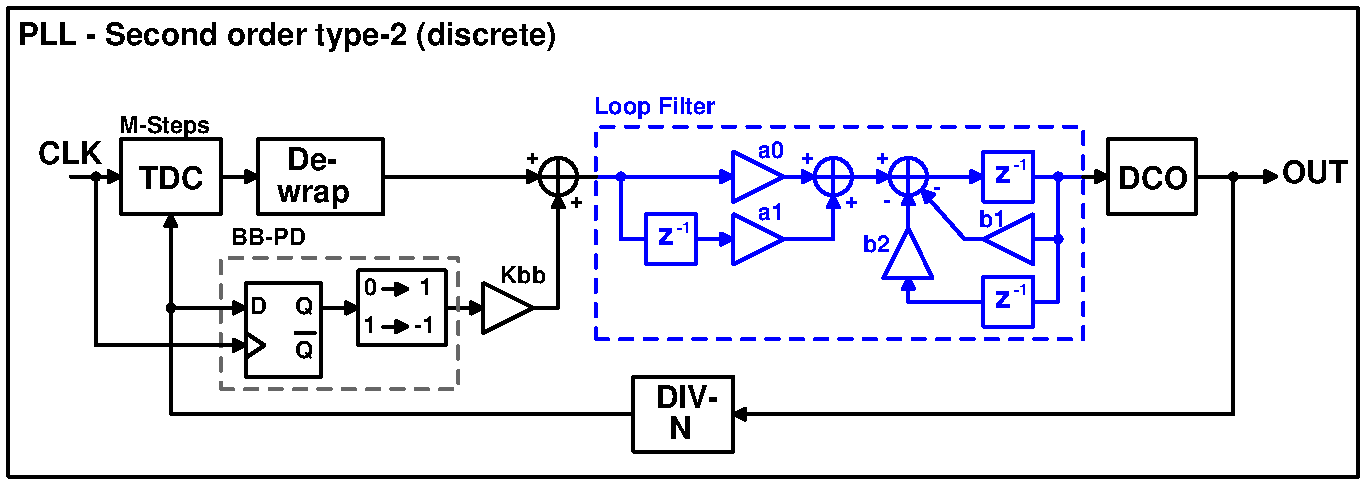
\includegraphics[width=0.8\textwidth, angle=0]{pll_sec_order_bb.pdf}

	\end{block}
		\begin{block}{Power Targets}
		\vspace{-.1em}
		\begin{table}[htb!]
			\tiny
			\centering
			\def\arraystretch{1.5}		
			\setlength\arrayrulewidth{0.75pt}
			\setlength{\tabcolsep}{1em} % for the horizontal padding
			\begin{tabular}{|l|l|l|l|l|}
				\hline 
				\rule[-1ex]{0pt}{2.5ex} \cellcolor{gray!40}\textbf{DCO} & \cellcolor{gray!40}\textbf{TDC} & \cellcolor{gray!40}\textbf{Divider }& \cellcolor{gray!40}\textbf{Other} & \cellcolor{gray!40}\textbf{SUM} \\ 
				\hline 
				\rule[-1ex]{0pt}{2.5ex} 70 $\mu$W& 20 $\mu$W & 10 $\mu$W & $<<$ 1 $\mu$W & 100 $\mu$W\\ 
				\hline 
			\end{tabular} 
			% \caption{Assigned specifications for branch line hybrid design.}
			% \label{asgn_specs}
		\end{table}   
	\end{block}

\end{frame}


% #############################################################################
% project phases
% #############################################################################


\begin{frame}
	\frametitle{Project Phases}
	\begin{block}{Autumn 2019}
		\footnotesize
		\begin{itemize}
			\item System modeling and simulation.
			\begin{itemize}
				\footnotesize
				\item Learn PLL theory in detail
				\item Evaluate feasability of PLL architectures (counter, TDC-based)
				\item Determine requirements for TDC/DCO/Divider/logic (bits of resolution, accuracy etc) to meet PLL performance specifications.
				\item Determine digital logic for loop filter, validate stability and lock time performance.
			\end{itemize}
			\item Research ultra-low power circuit topologies to implement system components that will meet determined requirements.
			\item Translate component-level specifications into schematic-level circuit designs.
			\begin{itemize}
				\footnotesize
				\item Try, fail, try again until functional at schematic level.
				\begin{itemize}
					\footnotesize
					\item I expect the TDC to be difficult.
				\end{itemize}
			\end{itemize}      
		\end{itemize}
	\end{block}
\end{frame}

% #############################################################################
% Project phases slide 2
% #############################################################################


\begin{frame}
	\frametitle{Project Phases (continued)}
	\begin{block}{Spring 2020}
		\begin{itemize}
			\footnotesize
			\item Finalize schematic-level design.
			\item Estabilish thorough tests for PLL performance (automated?) to help in layout.
			\item Layout of PLL.
			\begin{itemize}
				\footnotesize
				\item Design iteration until design specs met.
				\item Probably very time consuming.
			\end{itemize}
			\item Full characterization/validation of design performance. 
			\begin{itemize}
				\footnotesize
				\item Comprehensive Corners/Monte-Carlo testing (time consuming??)
				\item More design iteration if new issues crop up...
			\end{itemize}
			\item Thesis paper writing.
		\end{itemize}
	\end{block}
\end{frame}

% #############################################################################
% References
% #############################################################################


\begin{frame}
	\frametitle{References}
		\scriptsize
		[1] "Ultra-Low Power Wake-Up Receivers for Wireless Sensor Networks", N. Pletcher, J.M Rabaey, 2008.\\
		\hspace{16pt}\url{http://www.eecs.berkeley.edu/Pubs/TechRpts/2008/EECS-2008-59.html}\\
		\vspace{1em}
		% [2] "Minimum Achievable Phase Noise of RC Oscillators",
	% Navid et al. 2005
\end{frame}


\end{document}
